\documentclass[14pt]{beamer}
\usepackage{fancyvrb}
\RecustomVerbatimCommand{\VerbatimInput}{VerbatimInput}{frame=single,
numbersep=1mm, numbers=left, formatcom=\color{orange}}
%\usepackage{kpfonts}
%\usepackage[bitstream-charter]{mathdesign}
\usepackage[utf8]{inputenc}
\usepackage{pgf}
\usepackage{verbatim}
\usepackage{fontspec}
\usepackage[ruled,vlined,linesnumbered]{algorithm2e}
\IncMargin{1em}
\usetheme{Boadilla}
%\usecolortheme{fly}
\usecolortheme[dark]{solarized}
% \setsansfont{Ubuntu}
% \setmonofont{Ubuntu Mono}

\setbeamertemplate{blocks}[rounded][shadow=false]
\setbeamertemplate{navigation symbols}{}




% \usepackage{euler}
%\usepackage[T1]{fontenc}
\input{today.txt}

\author{Gianluca Della Vedova}
\title[Advanced Algorithms]{Advanced Techniques for Combinatorial Algorithms:
Introduction to Parallel Algorithms}

\institute[]{Univ. Milano--Bicocca\\
  \texttt{http://gianluca.dellavedova.org}}
\date[]{{\tiny \vcsDate\hspace{1em} \vcsShortHash}}

\DeclareMathOperator{\poly}{\text{poly}}
\DeclareMathOperator{\polylog}{\text{polylog}}


% If you wish to uncover everything in a step-wise fashion, uncomment
% the following command:
\beamerdefaultoverlayspecification{<+->}


\begin{document}

\begin{frame}
  \titlepage
\end{frame}


\begin{frame}\frametitle{Gianluca Della Vedova}
  \begin{itemize}
  \item
                Advanced Techniques for Combinatorial Algorithms
\item
{\small\url{https://gitlab.com/dellavg/advanced-algorithms}}
  \item
{\small\url{http://gianluca.dellavedova.org}}
  \item
{\small\url{gianluca.dellavedova@unimib.it}}
  \end{itemize}
\end{frame}



\begin{frame}\frametitle{RAM model}
  \begin{itemize}
  \item
    Random Access Memory
  \item
    One processor
  \item
    sequential algorithms
  \item
    Flat memory
  \item
    Infinite memory
  \end{itemize}
\end{frame}

\begin{frame}\frametitle{PRAM model}
  \begin{itemize}
  \item
    \alert{Parallel} RAM
  \item
    $p$ RAMs
  \item
    Shared memory
  \item
    Synchronized
  \end{itemize}
\end{frame}

\begin{frame}\frametitle{PRAM model}
  \begin{itemize}
  \item
Parallel computation is \alert{rapidly} becoming a \alert{dominant} theme in all areas of
computer science and its applications.
It is likely that, \alert{within a decade}, virtually all developments in computer
architecture, systems programming, computer applications and the design of
algorithms will be taking place within the context of parallel computation.
\item
\small  Karp, R M. and Ramachandran, V. Chapter 17. Parallel Algorithms for
  Shared-Memory Machines. Handbook of Theoretical Computer Science: Algorithms and complexity, Volume 1.
 \alert{1990}.
\end{itemize}
\end{frame}


\begin{frame}\frametitle{PRAM model}
\begin{references}
Selim Akl, Parallel Computation: Models and Methods, Prentice Hall, 1997.    
\end{references}

\begin{references}
Selim Akl, Design \& Analysis of Parallel Algorithms, Prentice Hall, 1989.
\end{references}

\begin{references}
Cormen, Leiserson, and Rivest, Introduction to Algorithms, 1st edition,
1990, McGraw Hill and MIT Press, Chapter 30 on parallel algorithms.
\end{references}

\begin{references}
Joseph JaJa, An Introduction to Parallel Algorithms, Addison Wesley, 1992.
\end{references}
\end{frame}

\begin{frame}\frametitle{PRAM model}
  \begin{itemize}
  \item
    It's a \alert{MODEL}!
  \item
    MIMD (Multiple Instruction Multiple Data)
  \item
    Processor ID
  \item
    No communication cost
  \end{itemize}
\end{frame}

\begin{frame}\frametitle{PRAM model}
% This LaTeX table template is generated by emacs 24.1.50.1
\begin{center}
  \begin{tabular}{|l|l|l|}
\hline
 & Read & Write \\
\hline
Exclusive & ER & EW \\
\hline
Concurrent & CR & CW \\
\hline
\end{tabular}

\begin{itemize}
\item
  Different accesses
  \item
    CRCW is better than EREW.
  \item
    But how much?
  \item
    Common CRCW: concurrent writes if same value from all processors
  \item
    Priority CRCW: highest priority processor wins
  \end{itemize}
\end{center}
\end{frame}


\begin{frame}\frametitle{Efficient Algorithm}
\begin{itemize}
\item
  $t(n)$ = polylogarithmic time
\item
  $p(n)$ = polynomial number of processors
\item
  $\mathbf{NC}$
\item
  $\mathbf{NC}\subseteq \mathbf{P}$
\item
  Hardness = $\mathbf{P}$-complete problems
\end{itemize}
\end{frame}


\begin{frame}\frametitle{Optimal Algorithm}
\begin{itemize}
\item
  \alert{work} $w(n) = t(n) p(n)$
\item
  $t(n)$ = polylogarithmic time
\item
  $w(n) = O(T(n))$, where $T(n)$ = time complexity of \alert{best known}
  sequential algorithm
\end{itemize}
\end{frame}


\begin{frame}\frametitle{Simulations}
\begin{itemize}
\item
  EREW PRAM can simulate CRCW PRAM
\item
  Time multiplied by $O(\log p(n))$
\end{itemize}
\end{frame}




\section{Algorithms}


\begin{frame}\frametitle{}
  \begin{center}
    \Huge
    Algorithms
  \end{center}
\end{frame}

\begin{frame}\frametitle{Prefix sum problem (PRAM)}
  \begin{itemize}
  \item
    Input
  \item
    Sequence $\langle x_{1}, \ldots , x_{n} \rangle$ of elements
  \item
    Associative operation $+$
  \item
    Output
  \item
     $S=\langle S_{1}  \ldots , S_{n} \rangle$, with $S_{i} = x_{1} +
     \cdots + x_{i}$
   \item
     trivial sequential algorithm
  \end{itemize}
\end{frame}

\begin{frame}\frametitle{Prefix sum}
\begin{algorithm}[H]
\SetKwData{Array}{$x_{1}, \ldots , x_{n}$}

\For{$i\gets 1$ \KwTo $n/2$ \uncover<2>{\alert{in parallel}}}
{
  $y_{i}\gets x_{2i-1} + x_{2i}$\;
}
$S^{*}_{i} = \text{PrefixSum}([y_{1}, \ldots , y_{n/2}])$\;
\tcc{$y_{i} = x_{1} + \cdots + x_{2i}$}
\For{$i\gets 1$ \KwTo $n$ \uncover<2>{\alert{in parallel}}}
{
  \If{$i$ is even}{
    $S_{i}\gets S^{*}_{i/2}$\;
  }
  \Else{
    $S_{i}\gets S^{*}_{i/2} + x_{i}$
  }
}
\caption{PrefixSum}
\end{algorithm}
\end{frame}


\begin{frame}\frametitle{Prefix sum}
  \begin{itemize}
  \item
    EREW
  \item
    $O(n)$ processors
  \item
    $w(n) = O(n\log n)$
  \item
    $O(n/\log n)$ processors are enough
  \end{itemize}

\begin{block}{Brent's scheduling principle}
  \begin{itemize}
  \item
    $t$ parallel steps on $p$ processors
  \item
    $p_{1}<p$
  \item
    $\lfloor p/p_{i}\rfloor +t$ parallel steps
  \end{itemize}
\end{block}
\end{frame}

\begin{frame}\frametitle{Find Maximum}
\begin{block}{Instance}
An array $A$ of $n$ integers
\end{block}
\begin{block}{Question}
Find the largest element in $A$.    
\end{block}
\begin{block}{Goal}
Fastest algorithm
\end{block}
\end{frame}

\begin{frame}\frametitle{Find Maximum}
\begin{algorithm}[H]
\SetKwData{Array}{$x_{1}, \ldots , x_{n}$}
\For{$i\gets 1$ \KwTo $n$ in parallel}{%
  $B[i]\gets $ true\;
}
\For{$i\gets 1$ \KwTo $n$ in parallel}{%
  \For{$j\gets 1$ \KwTo $n$ in parallel}{%
    \If{$A[i] < A[j]$ or $A[i] = A[j]$ and $i < j$}{%
      $B[i]\gets $ false\;
    }
  }
}
\For{$i\gets 1$ \KwTo $n$ in parallel}{%
  \If{$B[i]$}{Return $A[i]$}
}
\caption{Find1.    
Find Maximum in an Array $A$}
\end{algorithm}
Time? Work? 
\uncover<2>{\alert{$T(n)=O(1)$, $W(n)=O(n^{2})$}}
\end{frame}

\begin{frame}\frametitle{Find Maximum}
\begin{algorithm}[H]
\SetKwData{Array}{$x_{1}, \ldots , x_{n}$}
\eIf{$n > 16$}{%
  \For{$i\gets 1$ \KwTo $n$ in parallel}{%
    $B[i]\gets $Find2$(A[1 + \lfloor (i - 1)/\sqrt{n} \rfloor : \lfloor i/\sqrt{n} \rfloor])$\;
  }
  Find1($B$)\;
}{%
  Find1($A$)\;
}
\caption{Find2.    
Find Maximum in an Array $A$}
\end{algorithm}
$T(n)\le \sqrt{T(\sqrt{n})} + c_{1} \Rightarrow T(n) = O(\log \log n)$

$W(n)\le \sqrt{n} W(\sqrt{n}) + c_{2}n \Rightarrow W(n) = O(n \log \log n)$
\end{frame}


\begin{frame}\frametitle{Find Maximum}
\begin{algorithm}[H]
\SetKwData{Array}{$x_{1}, \ldots , x_{n}$}
\For{$i\gets 1$ \KwTo $n / \log\log n$ in parallel}{%
  $B[i]\gets \min(A[1 + \lfloor (i - 1)\log\log n \rfloor : \lfloor i/\log\log n
  \rfloor])$\;
}
Find2($B$)\;
\caption{Find3.    
Find Maximum in an Array $A$}
\end{algorithm}
$T(n) = O(\log \log n)$

$W(n) = O(n)$
\end{frame}


\begin{frame}\frametitle{Binary trees}
  \begin{itemize}
  \item
    Problem: to determine depth of each node
  \item
    parent, left child, right child
  \item
    $3$ processors for each node
  \item
    $O(n)$-time sequential algorithm
  \item
    Level-wise visit, each node in parallel
  \item
    $t(n)=$height
  \end{itemize}
\end{frame}


\begin{frame}\frametitle{Euler tour}
  \begin{center}
    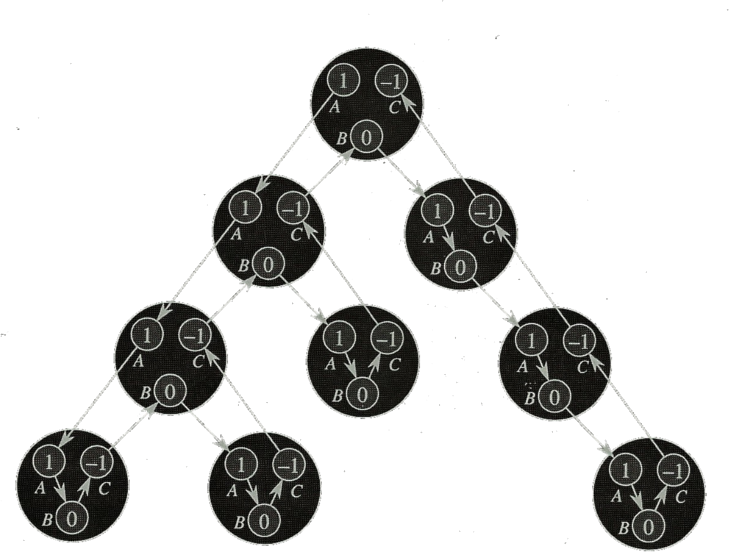
\includegraphics[width=8cm]{euler1.png}
  \end{center}

  \uncover<2>{Depth = prefix sum}
\end{frame}

\begin{frame}\frametitle{Graph Algorithms}
  \begin{itemize}
  \item
    depth-first visit
  \item
    No $\mathbf{NC}$ algorithm
  \item
    breadth-first visit
  \item
    $O(n^{2.37})$ processors
  \item
    \alert{Euler tour}
  \end{itemize}
\end{frame}


\begin{frame}\frametitle{Connected components}
\begin{block}{Instance}
Undirected graph $G=(V,E)$
\end{block}
\begin{block}{Data structure}
\begin{enumerate} 
\item
$M(v,w)$ adjacency matrix
\item
$R(v) \gets v$ representative.    
All vertices in the same connected components have the same representative.    
\item
$C[v,w]$ connected components with representative $v$ and $w$ can be merged
\end{enumerate}
\end{block}
\end{frame}

\begin{frame}\frametitle{Connected components}
  \begin{algorithm}[H]
    \ForEach{edge $(v,w)$ such that $R[v] \neq R[w]$}{
      \If{$R[v] < R[w]$}{%
        $C[R[v], R[w]] \gets $ true\;
      }
    }
    \ForEach{vertex $v$ such that $R[v]=v$}{
      $R[v] \gets \max w : C[R[v], R[w]]$ is true\;
    }
    \ForEach{vertex $v$}{
      $R[v] \gets R[R[v]]$\;
    }
    \caption{ConnectedComponents}
  \end{algorithm}
\end{frame}


\begin{frame}\frametitle{Minimum Spanning Tree}
\begin{block}{Problem}
Given an undirected edge-weighted connected graph $G=(V,E)$, find a
minimum-weight subset
$T\subseteq E$ such that $T$ is a tree spanning $V$.    
\end{block}

\begin{block}{Lemma}
Let $G=(V,E)$ be an undirected graph, let $(V_{1}, V_{2})$ be a
bipartition of $V$, let $T$ be a minimum spanning tree of $G$, and let
$e$ be the lightest edge connecting $V_{1}$ and $V_{2}$.    
Then $e\in T$.    
\end{block}
\end{frame}


\begin{frame}\frametitle{Additional Bibliography on PRAM}

\begin{references}
A Survey of Parallel Algorithms for Shared-Memory Machines
\url{http://techreports.lib.berkeley.edu/accessPages/CSD-88-408.html}
\end{references}

\begin{references}
Vishkin, Uzi (2009), Thinking in Parallel: Some Basic Data-Parallel Algorithms and
Techniques.    
\url{http://www.umiacs.umd.edu/users/vishkin/PUBLICATIONS/classnotes.pdf}    
\end{references}
\end{frame}


\end{document}

%%% Local Variables:
%%% mode: latex
%%% TeX-PDF-mode: t
%%% buffer-file-coding-system: utf-8
%%% End:
